\hypertarget{_lgm___sgp_8c}{
\section{/home/mgh/LanlGeoMag/libLanlGeoMag/Lgm\_\-Sgp.c File Reference}
\label{_lgm___sgp_8c}\index{/home/mgh/LanlGeoMag/libLanlGeoMag/Lgm\_\-Sgp.c@{/home/mgh/LanlGeoMag/libLanlGeoMag/Lgm\_\-Sgp.c}}
}
{\tt \#include \char`\"{}Lgm/Lgm\_\-CTrans.h\char`\"{}}\par
{\tt \#include \char`\"{}Lgm/Lgm\_\-Sgp.h\char`\"{}}\par
{\tt \#include $<$string.h$>$}\par
{\tt \#include $<$stdio.h$>$}\par
{\tt \#include $<$stdlib.h$>$}\par


Include dependency graph for Lgm\_\-Sgp.c:\nopagebreak
\begin{figure}[H]
\begin{center}
\leavevmode
\includegraphics[width=232pt]{_lgm___sgp_8c__incl}
\end{center}
\end{figure}
\subsection*{Functions}
\begin{CompactItemize}
\item 
int \hyperlink{_lgm___sgp_8c_6271ed7e00e88083593d9823dd3f5a9a}{LgmSgp\_\-TleChecksum} (char $\ast$Line)
\item 
int \hyperlink{_lgm___sgp_8c_21a21fc6d39baa848658e76b661a8063}{LgmSgp\_\-ReadTlesFromFile} (char $\ast$Filename, int $\ast$nTLEs, \hyperlink{struct___sgp_t_l_e}{\_\-SgpTLE} $\ast$TLEs, int Verbosity)
\item 
int \hyperlink{_lgm___sgp_8c_c8c62bf872785b575faa2f2c6093049a}{LgmSgp\_\-ReadTlesFromStrings} (char $\ast$Line0, char $\ast$Line1, char $\ast$Line2, int $\ast$nTLEs, \hyperlink{struct___sgp_t_l_e}{\_\-SgpTLE} $\ast$TLEs, int Verbosity)
\item 
void \hyperlink{_lgm___sgp_8c_1cdf495d9a7e1309a4b1ababdc14a64c}{Lgm\_\-SgpDecodeTle} (char $\ast$Line0, char $\ast$Line1, char $\ast$Line2, \hyperlink{struct___sgp_t_l_e}{\_\-SgpTLE} $\ast$TLE, int Verbosity)
\item 
double \hyperlink{_lgm___sgp_8c_4226a319104ba9b36b55e73a4c1d0d30}{LgmSgp\_\-gstime} (double jdut1)
\item 
void \hyperlink{_lgm___sgp_8c_3a3d1ab6587159dd6059bf83aa4b6924}{LgmSgp\_\-dpper} (double inclo, char init, double $\ast$ep, double $\ast$inclp, double $\ast$nodep, double $\ast$argpp, double $\ast$mp, \hyperlink{struct___sgp_info}{\_\-SgpInfo} $\ast$s)
\item 
void \hyperlink{_lgm___sgp_8c_584c10e9b76c3814acb6ac927d11dfdf}{LgmSgp\_\-dscom} (double epoch, double ep, double argpp, double tc, double inclp, double nodep, double np, double $\ast$snodm, double $\ast$cnodm, double $\ast$sinim, double $\ast$cosim, double $\ast$sinomm, double $\ast$cosomm, double $\ast$day, double $\ast$e3, double $\ast$ee2, double $\ast$em, double $\ast$emsq, double $\ast$gam, double $\ast$peo, double $\ast$pgho, double $\ast$pho, double $\ast$pinco, double $\ast$plo, double $\ast$rtemsq, double $\ast$se2, double $\ast$se3, double $\ast$sgh2, double $\ast$sgh3, double $\ast$sgh4, double $\ast$sh2, double $\ast$sh3, double $\ast$si2, double $\ast$si3, double $\ast$sl2, double $\ast$sl3, double $\ast$sl4, double $\ast$s1, double $\ast$s2, double $\ast$s3, double $\ast$s4, double $\ast$s5, double $\ast$s6, double $\ast$s7, double $\ast$ss1, double $\ast$ss2, double $\ast$ss3, double $\ast$ss4, double $\ast$ss5, double $\ast$ss6, double $\ast$ss7, double $\ast$sz1, double $\ast$sz2, double $\ast$sz3, double $\ast$sz11, double $\ast$sz12, double $\ast$sz13, double $\ast$sz21, double $\ast$sz22, double $\ast$sz23, double $\ast$sz31, double $\ast$sz32, double $\ast$sz33, double $\ast$xgh2, double $\ast$xgh3, double $\ast$xgh4, double $\ast$xh2, double $\ast$xh3, double $\ast$xi2, double $\ast$xi3, double $\ast$xl2, double $\ast$xl3, double $\ast$xl4, double $\ast$nm, double $\ast$z1, double $\ast$z2, double $\ast$z3, double $\ast$z11, double $\ast$z12, double $\ast$z13, double $\ast$z21, double $\ast$z22, double $\ast$z23, double $\ast$z31, double $\ast$z32, double $\ast$z33, double $\ast$zmol, double $\ast$zmos)
\item 
void \hyperlink{_lgm___sgp_8c_f068d9816c00ad56633a4dbfe8eb47b8}{LgmSgp\_\-dsinit} (int whichconst, double cosim, double emsq, double argpo, double s1, double s2, double s3, double s4, double s5, double sinim, double ss1, double ss2, double ss3, double ss4, double ss5, double sz1, double sz3, double sz11, double sz13, double sz21, double sz23, double sz31, double sz33, double t, double tc, double gsto, double mo, double mdot, double no, double nodeo, double nodedot, double xpidot, double z1, double z3, double z11, double z13, double z21, double z23, double z31, double z33, double ecco, double eccsq, double $\ast$em, double $\ast$argpm, double $\ast$inclm, double $\ast$mm, double $\ast$nm, double $\ast$nodem, int $\ast$irez, double $\ast$atime, double $\ast$d2201, double $\ast$d2211, double $\ast$d3210, double $\ast$d3222, double $\ast$d4410, double $\ast$d4422, double $\ast$d5220, double $\ast$d5232, double $\ast$d5421, double $\ast$d5433, double $\ast$dedt, double $\ast$didt, double $\ast$dmdt, double $\ast$dndt, double $\ast$dnodt, double $\ast$domdt, double $\ast$del1, double $\ast$del2, double $\ast$del3, double $\ast$xfact, double $\ast$xlamo, double $\ast$xli, double $\ast$xni)
\item 
void \hyperlink{_lgm___sgp_8c_58680584e882ac4b3357448060b030a8}{LgmSgp\_\-dspace} (double tc, double $\ast$atime, double $\ast$em, double $\ast$argpm, double $\ast$inclm, double $\ast$xli, double $\ast$mm, double $\ast$xni, double $\ast$nodem, double $\ast$dndt, double $\ast$nm, \hyperlink{struct___sgp_info}{\_\-SgpInfo} $\ast$s)
\item 
void \hyperlink{_lgm___sgp_8c_f3f227d3dbd22281b684cd11124b838d}{LgmSgp\_\-initl} (int satn, int whichconst, double ecco, double epoch, double inclo, double $\ast$no, char $\ast$method, double $\ast$ainv, double $\ast$ao, double $\ast$con41, double $\ast$con42, double $\ast$cosio, double $\ast$cosio2, double $\ast$eccsq, double $\ast$omeosq, double $\ast$posq, double $\ast$rp, double $\ast$rteosq, double $\ast$sinio, double $\ast$gsto)
\item 
int \hyperlink{_lgm___sgp_8c_19fa3cab6ea1bb0518dce1bb8c2b1c27}{LgmSgp\_\-SGP4\_\-Init} (\hyperlink{struct___sgp_info}{\_\-SgpInfo} $\ast$s, \hyperlink{struct___sgp_t_l_e}{\_\-SgpTLE} $\ast$t)
\item 
void \hyperlink{_lgm___sgp_8c_67d8f3b2acd5863c49efb5ba9e8c2eb7}{LgmSgp\_\-GetGravConst} (int whichconst, double $\ast$tumin, double $\ast$radiusearthkm, double $\ast$xke, double $\ast$j2, double $\ast$j3, double $\ast$j4, double $\ast$j3oj2)
\item 
int \hyperlink{_lgm___sgp_8c_35dcc38ab9090b839cb731cf751f6ad6}{LgmSgp\_\-SGP4} (double tsince, \hyperlink{struct___sgp_info}{\_\-SgpInfo} $\ast$s)
\end{CompactItemize}


\subsection{Function Documentation}
\hypertarget{_lgm___sgp_8c_6271ed7e00e88083593d9823dd3f5a9a}{
\index{Lgm\_\-Sgp.c@{Lgm\_\-Sgp.c}!LgmSgp\_\-TleChecksum@{LgmSgp\_\-TleChecksum}}
\index{LgmSgp\_\-TleChecksum@{LgmSgp\_\-TleChecksum}!Lgm_Sgp.c@{Lgm\_\-Sgp.c}}
\subsubsection[{LgmSgp\_\-TleChecksum}]{\setlength{\rightskip}{0pt plus 5cm}int LgmSgp\_\-TleChecksum (char $\ast$ {\em Line})}}
\label{_lgm___sgp_8c_6271ed7e00e88083593d9823dd3f5a9a}




Definition at line 10 of file Lgm\_\-Sgp.c.

Here is the caller graph for this function:\nopagebreak
\begin{figure}[H]
\begin{center}
\leavevmode
\includegraphics[width=175pt]{_lgm___sgp_8c_6271ed7e00e88083593d9823dd3f5a9a_icgraph}
\end{center}
\end{figure}
\hypertarget{_lgm___sgp_8c_21a21fc6d39baa848658e76b661a8063}{
\index{Lgm\_\-Sgp.c@{Lgm\_\-Sgp.c}!LgmSgp\_\-ReadTlesFromFile@{LgmSgp\_\-ReadTlesFromFile}}
\index{LgmSgp\_\-ReadTlesFromFile@{LgmSgp\_\-ReadTlesFromFile}!Lgm_Sgp.c@{Lgm\_\-Sgp.c}}
\subsubsection[{LgmSgp\_\-ReadTlesFromFile}]{\setlength{\rightskip}{0pt plus 5cm}int LgmSgp\_\-ReadTlesFromFile (char $\ast$ {\em Filename}, \/  int $\ast$ {\em nTLEs}, \/  {\bf \_\-SgpTLE} $\ast$ {\em TLEs}, \/  int {\em Verbosity})}}
\label{_lgm___sgp_8c_21a21fc6d39baa848658e76b661a8063}




Definition at line 27 of file Lgm\_\-Sgp.c.

Here is the call graph for this function:\nopagebreak
\begin{figure}[H]
\begin{center}
\leavevmode
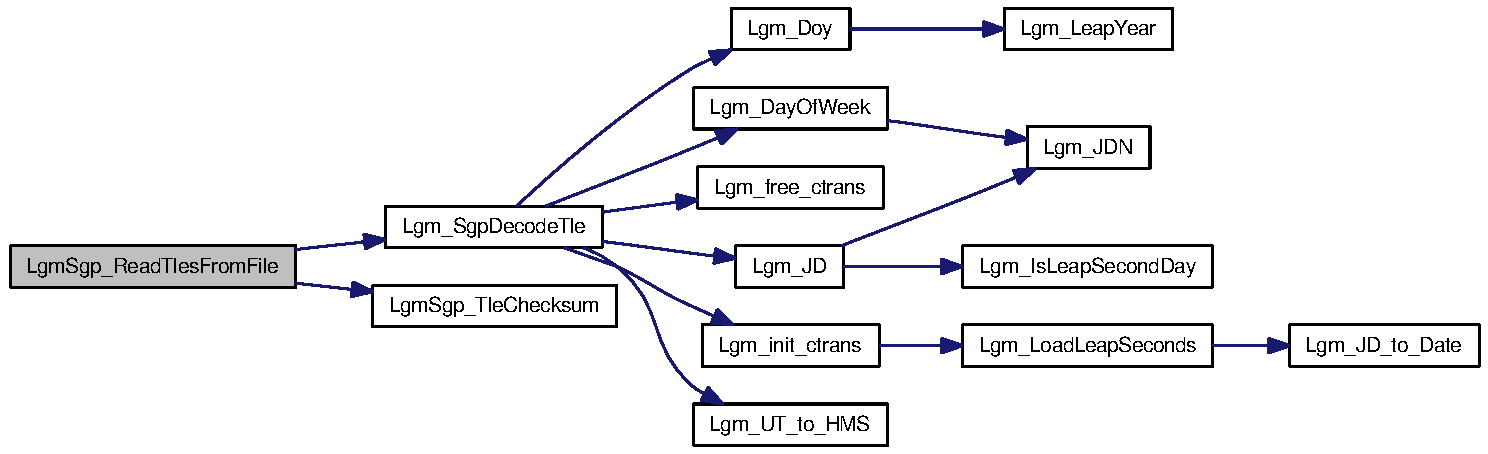
\includegraphics[width=375pt]{_lgm___sgp_8c_21a21fc6d39baa848658e76b661a8063_cgraph}
\end{center}
\end{figure}
\hypertarget{_lgm___sgp_8c_c8c62bf872785b575faa2f2c6093049a}{
\index{Lgm\_\-Sgp.c@{Lgm\_\-Sgp.c}!LgmSgp\_\-ReadTlesFromStrings@{LgmSgp\_\-ReadTlesFromStrings}}
\index{LgmSgp\_\-ReadTlesFromStrings@{LgmSgp\_\-ReadTlesFromStrings}!Lgm_Sgp.c@{Lgm\_\-Sgp.c}}
\subsubsection[{LgmSgp\_\-ReadTlesFromStrings}]{\setlength{\rightskip}{0pt plus 5cm}int LgmSgp\_\-ReadTlesFromStrings (char $\ast$ {\em Line0}, \/  char $\ast$ {\em Line1}, \/  char $\ast$ {\em Line2}, \/  int $\ast$ {\em nTLEs}, \/  {\bf \_\-SgpTLE} $\ast$ {\em TLEs}, \/  int {\em Verbosity})}}
\label{_lgm___sgp_8c_c8c62bf872785b575faa2f2c6093049a}




Definition at line 151 of file Lgm\_\-Sgp.c.

Here is the call graph for this function:\nopagebreak
\begin{figure}[H]
\begin{center}
\leavevmode
\includegraphics[width=382pt]{_lgm___sgp_8c_c8c62bf872785b575faa2f2c6093049a_cgraph}
\end{center}
\end{figure}
\hypertarget{_lgm___sgp_8c_1cdf495d9a7e1309a4b1ababdc14a64c}{
\index{Lgm\_\-Sgp.c@{Lgm\_\-Sgp.c}!Lgm\_\-SgpDecodeTle@{Lgm\_\-SgpDecodeTle}}
\index{Lgm\_\-SgpDecodeTle@{Lgm\_\-SgpDecodeTle}!Lgm_Sgp.c@{Lgm\_\-Sgp.c}}
\subsubsection[{Lgm\_\-SgpDecodeTle}]{\setlength{\rightskip}{0pt plus 5cm}void Lgm\_\-SgpDecodeTle (char $\ast$ {\em Line0}, \/  char $\ast$ {\em Line1}, \/  char $\ast$ {\em Line2}, \/  {\bf \_\-SgpTLE} $\ast$ {\em TLE}, \/  int {\em Verbosity})}}
\label{_lgm___sgp_8c_1cdf495d9a7e1309a4b1ababdc14a64c}




Definition at line 239 of file Lgm\_\-Sgp.c.

Here is the call graph for this function:\nopagebreak
\begin{figure}[H]
\begin{center}
\leavevmode
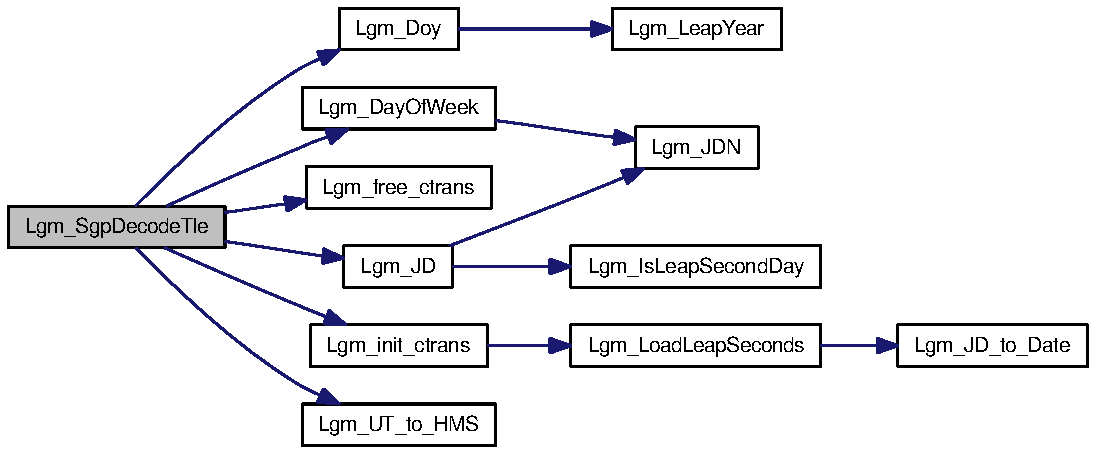
\includegraphics[width=281pt]{_lgm___sgp_8c_1cdf495d9a7e1309a4b1ababdc14a64c_cgraph}
\end{center}
\end{figure}


Here is the caller graph for this function:\nopagebreak
\begin{figure}[H]
\begin{center}
\leavevmode
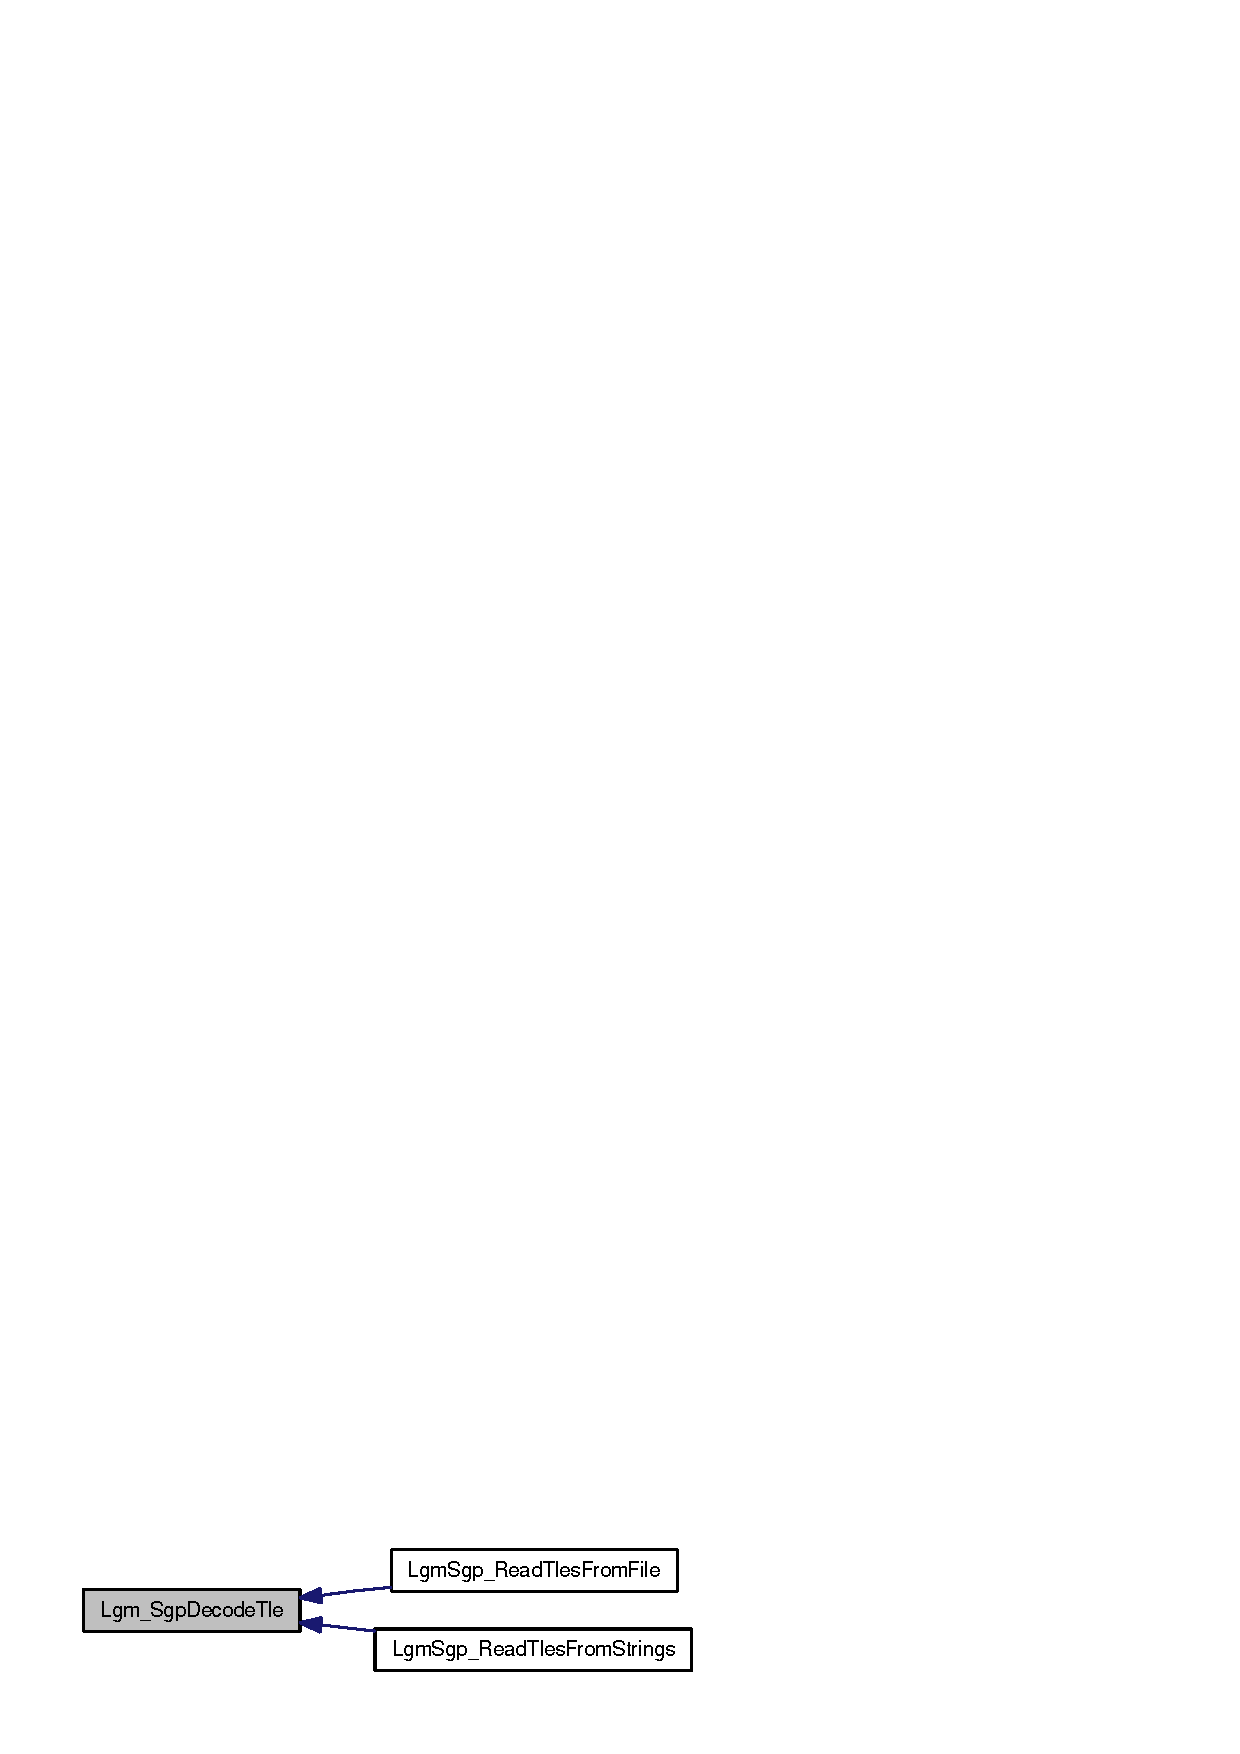
\includegraphics[width=168pt]{_lgm___sgp_8c_1cdf495d9a7e1309a4b1ababdc14a64c_icgraph}
\end{center}
\end{figure}
\hypertarget{_lgm___sgp_8c_4226a319104ba9b36b55e73a4c1d0d30}{
\index{Lgm\_\-Sgp.c@{Lgm\_\-Sgp.c}!LgmSgp\_\-gstime@{LgmSgp\_\-gstime}}
\index{LgmSgp\_\-gstime@{LgmSgp\_\-gstime}!Lgm_Sgp.c@{Lgm\_\-Sgp.c}}
\subsubsection[{LgmSgp\_\-gstime}]{\setlength{\rightskip}{0pt plus 5cm}double LgmSgp\_\-gstime (double {\em jdut1})}}
\label{_lgm___sgp_8c_4226a319104ba9b36b55e73a4c1d0d30}




Definition at line 414 of file Lgm\_\-Sgp.c.

Here is the caller graph for this function:\nopagebreak
\begin{figure}[H]
\begin{center}
\leavevmode
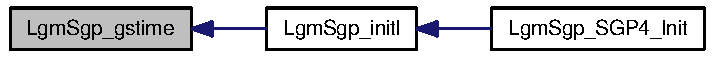
\includegraphics[width=189pt]{_lgm___sgp_8c_4226a319104ba9b36b55e73a4c1d0d30_icgraph}
\end{center}
\end{figure}
\hypertarget{_lgm___sgp_8c_3a3d1ab6587159dd6059bf83aa4b6924}{
\index{Lgm\_\-Sgp.c@{Lgm\_\-Sgp.c}!LgmSgp\_\-dpper@{LgmSgp\_\-dpper}}
\index{LgmSgp\_\-dpper@{LgmSgp\_\-dpper}!Lgm_Sgp.c@{Lgm\_\-Sgp.c}}
\subsubsection[{LgmSgp\_\-dpper}]{\setlength{\rightskip}{0pt plus 5cm}void LgmSgp\_\-dpper (double {\em inclo}, \/  char {\em init}, \/  double $\ast$ {\em ep}, \/  double $\ast$ {\em inclp}, \/  double $\ast$ {\em nodep}, \/  double $\ast$ {\em argpp}, \/  double $\ast$ {\em mp}, \/  {\bf \_\-SgpInfo} $\ast$ {\em s})}}
\label{_lgm___sgp_8c_3a3d1ab6587159dd6059bf83aa4b6924}




Definition at line 462 of file Lgm\_\-Sgp.c.

Here is the caller graph for this function:\nopagebreak
\begin{figure}[H]
\begin{center}
\leavevmode
\includegraphics[width=192pt]{_lgm___sgp_8c_3a3d1ab6587159dd6059bf83aa4b6924_icgraph}
\end{center}
\end{figure}
\hypertarget{_lgm___sgp_8c_584c10e9b76c3814acb6ac927d11dfdf}{
\index{Lgm\_\-Sgp.c@{Lgm\_\-Sgp.c}!LgmSgp\_\-dscom@{LgmSgp\_\-dscom}}
\index{LgmSgp\_\-dscom@{LgmSgp\_\-dscom}!Lgm_Sgp.c@{Lgm\_\-Sgp.c}}
\subsubsection[{LgmSgp\_\-dscom}]{\setlength{\rightskip}{0pt plus 5cm}void LgmSgp\_\-dscom (double {\em epoch}, \/  double {\em ep}, \/  double {\em argpp}, \/  double {\em tc}, \/  double {\em inclp}, \/  double {\em nodep}, \/  double {\em np}, \/  double $\ast$ {\em snodm}, \/  double $\ast$ {\em cnodm}, \/  double $\ast$ {\em sinim}, \/  double $\ast$ {\em cosim}, \/  double $\ast$ {\em sinomm}, \/  double $\ast$ {\em cosomm}, \/  double $\ast$ {\em day}, \/  double $\ast$ {\em e3}, \/  double $\ast$ {\em ee2}, \/  double $\ast$ {\em em}, \/  double $\ast$ {\em emsq}, \/  double $\ast$ {\em gam}, \/  double $\ast$ {\em peo}, \/  double $\ast$ {\em pgho}, \/  double $\ast$ {\em pho}, \/  double $\ast$ {\em pinco}, \/  double $\ast$ {\em plo}, \/  double $\ast$ {\em rtemsq}, \/  double $\ast$ {\em se2}, \/  double $\ast$ {\em se3}, \/  double $\ast$ {\em sgh2}, \/  double $\ast$ {\em sgh3}, \/  double $\ast$ {\em sgh4}, \/  double $\ast$ {\em sh2}, \/  double $\ast$ {\em sh3}, \/  double $\ast$ {\em si2}, \/  double $\ast$ {\em si3}, \/  double $\ast$ {\em sl2}, \/  double $\ast$ {\em sl3}, \/  double $\ast$ {\em sl4}, \/  double $\ast$ {\em s1}, \/  double $\ast$ {\em s2}, \/  double $\ast$ {\em s3}, \/  double $\ast$ {\em s4}, \/  double $\ast$ {\em s5}, \/  double $\ast$ {\em s6}, \/  double $\ast$ {\em s7}, \/  double $\ast$ {\em ss1}, \/  double $\ast$ {\em ss2}, \/  double $\ast$ {\em ss3}, \/  double $\ast$ {\em ss4}, \/  double $\ast$ {\em ss5}, \/  double $\ast$ {\em ss6}, \/  double $\ast$ {\em ss7}, \/  double $\ast$ {\em sz1}, \/  double $\ast$ {\em sz2}, \/  double $\ast$ {\em sz3}, \/  double $\ast$ {\em sz11}, \/  double $\ast$ {\em sz12}, \/  double $\ast$ {\em sz13}, \/  double $\ast$ {\em sz21}, \/  double $\ast$ {\em sz22}, \/  double $\ast$ {\em sz23}, \/  double $\ast$ {\em sz31}, \/  double $\ast$ {\em sz32}, \/  double $\ast$ {\em sz33}, \/  double $\ast$ {\em xgh2}, \/  double $\ast$ {\em xgh3}, \/  double $\ast$ {\em xgh4}, \/  double $\ast$ {\em xh2}, \/  double $\ast$ {\em xh3}, \/  double $\ast$ {\em xi2}, \/  double $\ast$ {\em xi3}, \/  double $\ast$ {\em xl2}, \/  double $\ast$ {\em xl3}, \/  double $\ast$ {\em xl4}, \/  double $\ast$ {\em nm}, \/  double $\ast$ {\em z1}, \/  double $\ast$ {\em z2}, \/  double $\ast$ {\em z3}, \/  double $\ast$ {\em z11}, \/  double $\ast$ {\em z12}, \/  double $\ast$ {\em z13}, \/  double $\ast$ {\em z21}, \/  double $\ast$ {\em z22}, \/  double $\ast$ {\em z23}, \/  double $\ast$ {\em z31}, \/  double $\ast$ {\em z32}, \/  double $\ast$ {\em z33}, \/  double $\ast$ {\em zmol}, \/  double $\ast$ {\em zmos})}}
\label{_lgm___sgp_8c_584c10e9b76c3814acb6ac927d11dfdf}




Definition at line 649 of file Lgm\_\-Sgp.c.

Here is the caller graph for this function:\nopagebreak
\begin{figure}[H]
\begin{center}
\leavevmode
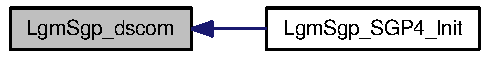
\includegraphics[width=135pt]{_lgm___sgp_8c_584c10e9b76c3814acb6ac927d11dfdf_icgraph}
\end{center}
\end{figure}
\hypertarget{_lgm___sgp_8c_f068d9816c00ad56633a4dbfe8eb47b8}{
\index{Lgm\_\-Sgp.c@{Lgm\_\-Sgp.c}!LgmSgp\_\-dsinit@{LgmSgp\_\-dsinit}}
\index{LgmSgp\_\-dsinit@{LgmSgp\_\-dsinit}!Lgm_Sgp.c@{Lgm\_\-Sgp.c}}
\subsubsection[{LgmSgp\_\-dsinit}]{\setlength{\rightskip}{0pt plus 5cm}void LgmSgp\_\-dsinit (int {\em whichconst}, \/  double {\em cosim}, \/  double {\em emsq}, \/  double {\em argpo}, \/  double {\em s1}, \/  double {\em s2}, \/  double {\em s3}, \/  double {\em s4}, \/  double {\em s5}, \/  double {\em sinim}, \/  double {\em ss1}, \/  double {\em ss2}, \/  double {\em ss3}, \/  double {\em ss4}, \/  double {\em ss5}, \/  double {\em sz1}, \/  double {\em sz3}, \/  double {\em sz11}, \/  double {\em sz13}, \/  double {\em sz21}, \/  double {\em sz23}, \/  double {\em sz31}, \/  double {\em sz33}, \/  double {\em t}, \/  double {\em tc}, \/  double {\em gsto}, \/  double {\em mo}, \/  double {\em mdot}, \/  double {\em no}, \/  double {\em nodeo}, \/  double {\em nodedot}, \/  double {\em xpidot}, \/  double {\em z1}, \/  double {\em z3}, \/  double {\em z11}, \/  double {\em z13}, \/  double {\em z21}, \/  double {\em z23}, \/  double {\em z31}, \/  double {\em z33}, \/  double {\em ecco}, \/  double {\em eccsq}, \/  double $\ast$ {\em em}, \/  double $\ast$ {\em argpm}, \/  double $\ast$ {\em inclm}, \/  double $\ast$ {\em mm}, \/  double $\ast$ {\em nm}, \/  double $\ast$ {\em nodem}, \/  int $\ast$ {\em irez}, \/  double $\ast$ {\em atime}, \/  double $\ast$ {\em d2201}, \/  double $\ast$ {\em d2211}, \/  double $\ast$ {\em d3210}, \/  double $\ast$ {\em d3222}, \/  double $\ast$ {\em d4410}, \/  double $\ast$ {\em d4422}, \/  double $\ast$ {\em d5220}, \/  double $\ast$ {\em d5232}, \/  double $\ast$ {\em d5421}, \/  double $\ast$ {\em d5433}, \/  double $\ast$ {\em dedt}, \/  double $\ast$ {\em didt}, \/  double $\ast$ {\em dmdt}, \/  double $\ast$ {\em dndt}, \/  double $\ast$ {\em dnodt}, \/  double $\ast$ {\em domdt}, \/  double $\ast$ {\em del1}, \/  double $\ast$ {\em del2}, \/  double $\ast$ {\em del3}, \/  double $\ast$ {\em xfact}, \/  double $\ast$ {\em xlamo}, \/  double $\ast$ {\em xli}, \/  double $\ast$ {\em xni})}}
\label{_lgm___sgp_8c_f068d9816c00ad56633a4dbfe8eb47b8}




Definition at line 902 of file Lgm\_\-Sgp.c.

Here is the call graph for this function:\nopagebreak
\begin{figure}[H]
\begin{center}
\leavevmode
\includegraphics[width=141pt]{_lgm___sgp_8c_f068d9816c00ad56633a4dbfe8eb47b8_cgraph}
\end{center}
\end{figure}


Here is the caller graph for this function:\nopagebreak
\begin{figure}[H]
\begin{center}
\leavevmode
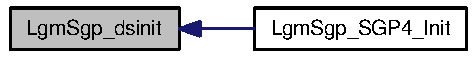
\includegraphics[width=132pt]{_lgm___sgp_8c_f068d9816c00ad56633a4dbfe8eb47b8_icgraph}
\end{center}
\end{figure}
\hypertarget{_lgm___sgp_8c_58680584e882ac4b3357448060b030a8}{
\index{Lgm\_\-Sgp.c@{Lgm\_\-Sgp.c}!LgmSgp\_\-dspace@{LgmSgp\_\-dspace}}
\index{LgmSgp\_\-dspace@{LgmSgp\_\-dspace}!Lgm_Sgp.c@{Lgm\_\-Sgp.c}}
\subsubsection[{LgmSgp\_\-dspace}]{\setlength{\rightskip}{0pt plus 5cm}void LgmSgp\_\-dspace (double {\em tc}, \/  double $\ast$ {\em atime}, \/  double $\ast$ {\em em}, \/  double $\ast$ {\em argpm}, \/  double $\ast$ {\em inclm}, \/  double $\ast$ {\em xli}, \/  double $\ast$ {\em mm}, \/  double $\ast$ {\em xni}, \/  double $\ast$ {\em nodem}, \/  double $\ast$ {\em dndt}, \/  double $\ast$ {\em nm}, \/  {\bf \_\-SgpInfo} $\ast$ {\em s})}}
\label{_lgm___sgp_8c_58680584e882ac4b3357448060b030a8}




Definition at line 1176 of file Lgm\_\-Sgp.c.

Here is the caller graph for this function:\nopagebreak
\begin{figure}[H]
\begin{center}
\leavevmode
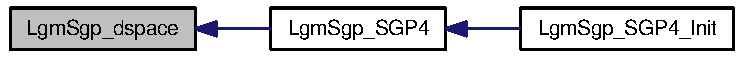
\includegraphics[width=196pt]{_lgm___sgp_8c_58680584e882ac4b3357448060b030a8_icgraph}
\end{center}
\end{figure}
\hypertarget{_lgm___sgp_8c_f3f227d3dbd22281b684cd11124b838d}{
\index{Lgm\_\-Sgp.c@{Lgm\_\-Sgp.c}!LgmSgp\_\-initl@{LgmSgp\_\-initl}}
\index{LgmSgp\_\-initl@{LgmSgp\_\-initl}!Lgm_Sgp.c@{Lgm\_\-Sgp.c}}
\subsubsection[{LgmSgp\_\-initl}]{\setlength{\rightskip}{0pt plus 5cm}void LgmSgp\_\-initl (int {\em satn}, \/  int {\em whichconst}, \/  double {\em ecco}, \/  double {\em epoch}, \/  double {\em inclo}, \/  double $\ast$ {\em no}, \/  char $\ast$ {\em method}, \/  double $\ast$ {\em ainv}, \/  double $\ast$ {\em ao}, \/  double $\ast$ {\em con41}, \/  double $\ast$ {\em con42}, \/  double $\ast$ {\em cosio}, \/  double $\ast$ {\em cosio2}, \/  double $\ast$ {\em eccsq}, \/  double $\ast$ {\em omeosq}, \/  double $\ast$ {\em posq}, \/  double $\ast$ {\em rp}, \/  double $\ast$ {\em rteosq}, \/  double $\ast$ {\em sinio}, \/  double $\ast$ {\em gsto})}}
\label{_lgm___sgp_8c_f3f227d3dbd22281b684cd11124b838d}




Definition at line 1365 of file Lgm\_\-Sgp.c.

Here is the call graph for this function:\nopagebreak
\begin{figure}[H]
\begin{center}
\leavevmode
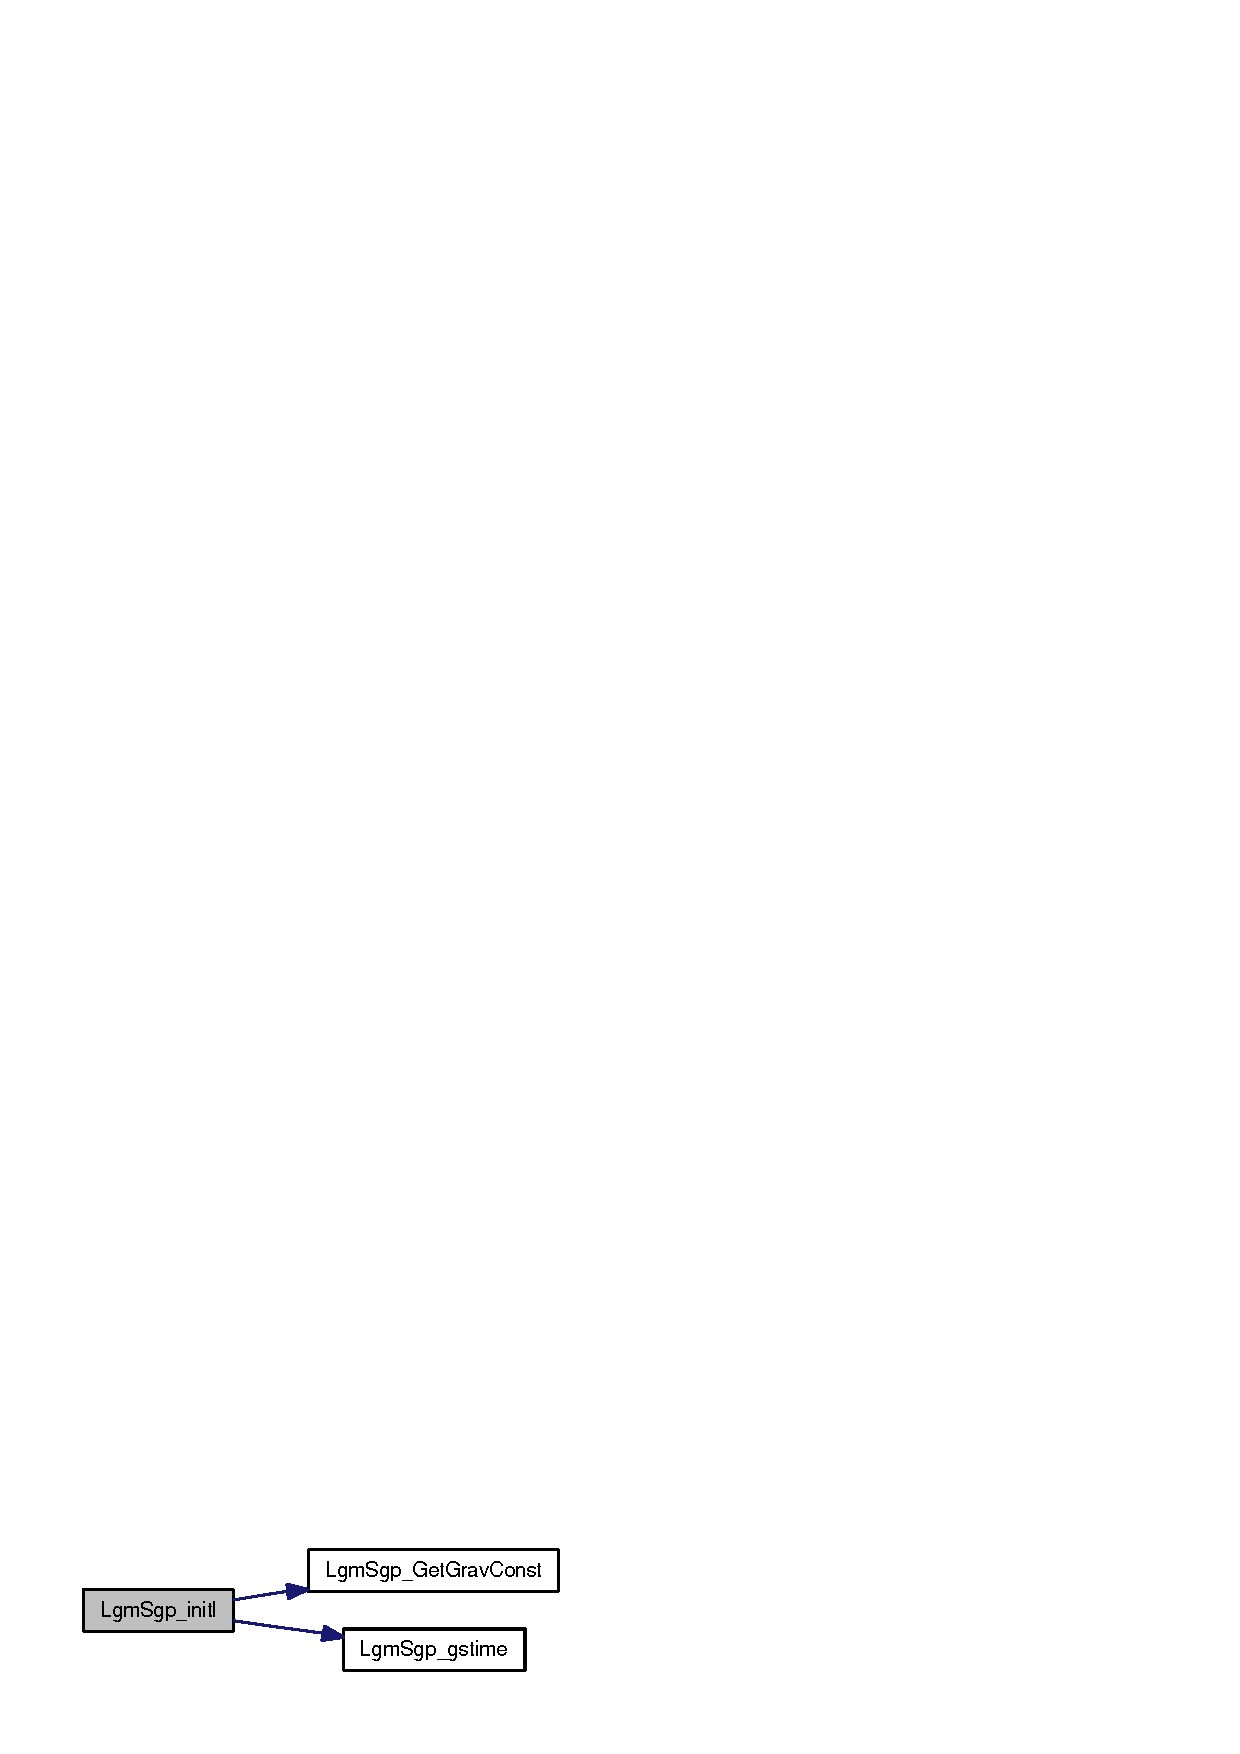
\includegraphics[width=136pt]{_lgm___sgp_8c_f3f227d3dbd22281b684cd11124b838d_cgraph}
\end{center}
\end{figure}


Here is the caller graph for this function:\nopagebreak
\begin{figure}[H]
\begin{center}
\leavevmode
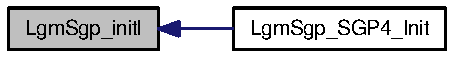
\includegraphics[width=127pt]{_lgm___sgp_8c_f3f227d3dbd22281b684cd11124b838d_icgraph}
\end{center}
\end{figure}
\hypertarget{_lgm___sgp_8c_19fa3cab6ea1bb0518dce1bb8c2b1c27}{
\index{Lgm\_\-Sgp.c@{Lgm\_\-Sgp.c}!LgmSgp\_\-SGP4\_\-Init@{LgmSgp\_\-SGP4\_\-Init}}
\index{LgmSgp\_\-SGP4\_\-Init@{LgmSgp\_\-SGP4\_\-Init}!Lgm_Sgp.c@{Lgm\_\-Sgp.c}}
\subsubsection[{LgmSgp\_\-SGP4\_\-Init}]{\setlength{\rightskip}{0pt plus 5cm}int LgmSgp\_\-SGP4\_\-Init ({\bf \_\-SgpInfo} $\ast$ {\em s}, \/  {\bf \_\-SgpTLE} $\ast$ {\em t})}}
\label{_lgm___sgp_8c_19fa3cab6ea1bb0518dce1bb8c2b1c27}




Definition at line 1461 of file Lgm\_\-Sgp.c.

Here is the call graph for this function:\nopagebreak
\begin{figure}[H]
\begin{center}
\leavevmode
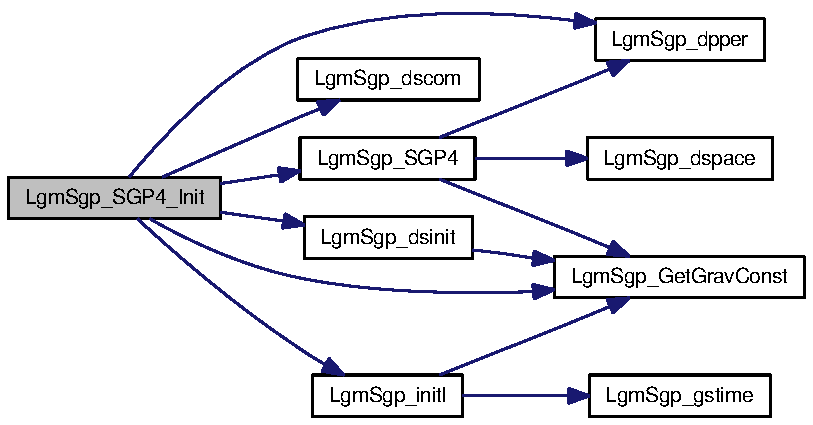
\includegraphics[width=213pt]{_lgm___sgp_8c_19fa3cab6ea1bb0518dce1bb8c2b1c27_cgraph}
\end{center}
\end{figure}
\hypertarget{_lgm___sgp_8c_67d8f3b2acd5863c49efb5ba9e8c2eb7}{
\index{Lgm\_\-Sgp.c@{Lgm\_\-Sgp.c}!LgmSgp\_\-GetGravConst@{LgmSgp\_\-GetGravConst}}
\index{LgmSgp\_\-GetGravConst@{LgmSgp\_\-GetGravConst}!Lgm_Sgp.c@{Lgm\_\-Sgp.c}}
\subsubsection[{LgmSgp\_\-GetGravConst}]{\setlength{\rightskip}{0pt plus 5cm}void LgmSgp\_\-GetGravConst (int {\em whichconst}, \/  double $\ast$ {\em tumin}, \/  double $\ast$ {\em radiusearthkm}, \/  double $\ast$ {\em xke}, \/  double $\ast$ {\em j2}, \/  double $\ast$ {\em j3}, \/  double $\ast$ {\em j4}, \/  double $\ast$ {\em j3oj2})}}
\label{_lgm___sgp_8c_67d8f3b2acd5863c49efb5ba9e8c2eb7}




Definition at line 1740 of file Lgm\_\-Sgp.c.

Here is the caller graph for this function:\nopagebreak
\begin{figure}[H]
\begin{center}
\leavevmode
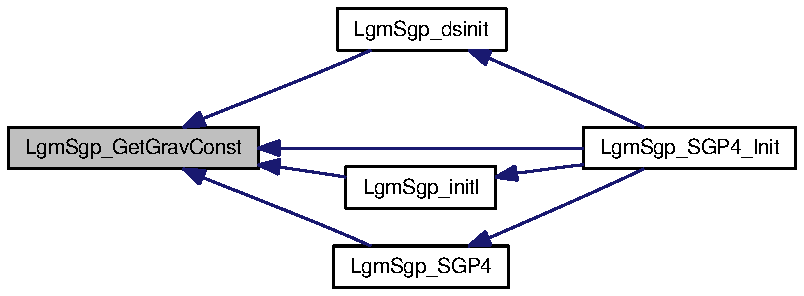
\includegraphics[width=211pt]{_lgm___sgp_8c_67d8f3b2acd5863c49efb5ba9e8c2eb7_icgraph}
\end{center}
\end{figure}
\hypertarget{_lgm___sgp_8c_35dcc38ab9090b839cb731cf751f6ad6}{
\index{Lgm\_\-Sgp.c@{Lgm\_\-Sgp.c}!LgmSgp\_\-SGP4@{LgmSgp\_\-SGP4}}
\index{LgmSgp\_\-SGP4@{LgmSgp\_\-SGP4}!Lgm_Sgp.c@{Lgm\_\-Sgp.c}}
\subsubsection[{LgmSgp\_\-SGP4}]{\setlength{\rightskip}{0pt plus 5cm}int LgmSgp\_\-SGP4 (double {\em tsince}, \/  {\bf \_\-SgpInfo} $\ast$ {\em s})}}
\label{_lgm___sgp_8c_35dcc38ab9090b839cb731cf751f6ad6}




Definition at line 1842 of file Lgm\_\-Sgp.c.

Here is the call graph for this function:\nopagebreak
\begin{figure}[H]
\begin{center}
\leavevmode
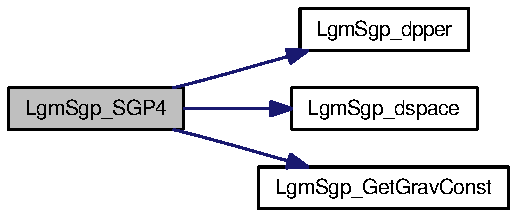
\includegraphics[width=142pt]{_lgm___sgp_8c_35dcc38ab9090b839cb731cf751f6ad6_cgraph}
\end{center}
\end{figure}


Here is the caller graph for this function:\nopagebreak
\begin{figure}[H]
\begin{center}
\leavevmode
\includegraphics[width=133pt]{_lgm___sgp_8c_35dcc38ab9090b839cb731cf751f6ad6_icgraph}
\end{center}
\end{figure}
